\documentclass[conference]{IEEEtran}
\usepackage[boxed,commentsnumbered]{algorithm2e}
\usepackage{graphicx}
\usepackage{xcolor}
\usepackage{soul}
\usepackage{supertabular}
\usepackage{tabularx}
\usepackage{ caption, floatrow, makecell, booktabs}%
\usepackage{hyperref}
\hypersetup{
    colorlinks=true,
    linkcolor=black,
    citecolor=black,
    urlcolor=blue,
}
\setcounter{tocdepth}{1}
\usepackage{pdfpages}
\newcommand{\hlc}[2][yellow]{{%
    \colorlet{foo}{#1}%
    \sethlcolor{foo}\hl{#2}}%
}
\title{Analysing Algorithmic Patterns Based on Real Coding Interview Questions}
\author{
\IEEEauthorblockN{Ian Dempsey}
\IEEEauthorblockA{Computer Science Department, \\
Maynooth University,\\
Email: ian.dempsey.2013@mumail.ie}
\and
\IEEEauthorblockN{Supervisor: Hao Wu}
\IEEEauthorblockA{Computer Science Department, \\
Maynooth University,\\
Email: haowu@cs.nuim.ie}
}

%\hlc[cyan!50]{_____} -> put in the stuff to be highlighted inside the {}
%cite{___} ->put in the bibtex key for the specific source.
%\label{sec: | fig: | } -> use to give something a specific label. This allows it to be referenced later
%\ref{___} -> to refernce a previously labeled area
\begin{document}
\tableofcontents
\addtocontents{toc}{~\hfill\textbf{Page}\par}
\listoffigures
\listoftables
\newpage
\maketitle
\pagenumbering{gobble}
\newpage
\pagenumbering{arabic}
\begin{abstract}
This thesis aims to analyse algorithmic patterns based on real coding interview questions. This is because programming questions have become staples in any interview with technology companies. To perform detailed analysis, we first select a small set of highly used interview questions, simulate and complete each question within restrictive time allowances. This allows the solutions created to be as authentic as possible. We then plot control flow graphs for each selected question and identify the pattern by highlighting the key differences in different algorithms. Further, this thesis shows that mastering a small set of questions allows interviewees to prepare a wide range of key topics to be interviewed. Thus, the identified patterns are important and can be used to save a significant amount of time on preparing long and exhausting coding practice before the interview.
\end{abstract}
\section{Introduction}
\label{sec:intro}
Nowadays interviews for jobs in the I.T industry are becoming more complex and demanding on the applicant. As this section of the working industry is usually quite technical, it is quite common for the applicants to perform some form of technical tests. These tests normally involve several questions that are based on a wide variety of topics in algorithms and data structures. These types of interview questions typically require a candidate to understand and analyse questions, then write a piece of code that is bug-free. This is quite challenging and demanding for an even experienced programmer. To prepare this kind of interview, a candidate usually goes through as many algorithmic questions as possible. This process is very time consuming and not easy to manage as a question bank usually has more than 500 questions and many of them are very challenging. They require a candidate to go over solutions multiple times to truly master them.

The purpose of this thesis is to study the relationship between the standard (fundamental) algorithms and the interview questions that are commonly asked. This thesis aims to give a guidance to people who are willing to spend much less time on preparing the interview questions and in the meanwhile cover a wide range of frequently interviewed topics.

This thesis presents a study that summarises the similarities between interview questions and standard algorithms taught in a standard programming course. This distinguishes our work from interview preparation books which focus on the problem-solving skills, simply showing the reader a solution to a single problem, and not reinforcing material they would already be familiar with.


The contribution of this thesis can be summarised as the following: 
\begin{itemize}
\item[1.] We view mastering the fundamental algorithms as a key to cover a wide range of real world interview questions. 
\item[2.] We identify patterns that are closely related to these standard algorithms. 
\item[3.] We believe that this thesis can be used as a guidance for fresh graduates which can prepare them for real world interview questions.  
\end{itemize}
\section{Background}
In general, there are quite a lot of online repositories showing interview questions and interview related material. For example, websites like hackerrank.com, glassdoor.ie, geeksforgeeks.org, and leetcode.com offer information on what questions are common during interviews for different companies. These websites also provide an online judge system to run potential solutions to some of the given questions. 

For this thesis we choose to use leetcode.com\cite{leet1}, as this website comes with a huge amount of online material that is taken from previously asked interview questions. Companies also use sites similar to LeetCode when they are building up a bank of questions to pose to candidates. This is important in our decision for the repository, as it means that we are using a platform that is regularly updated. LeetCode itself also has built-in features that greatly appeal to us. The website has an online discussion forum for each question, allowing the community to discuss solutions, issues, and the interview questions themselves. LeetCode host their own weekly coding competitions that allow users to gain more experience and confidence in coding problems. One of the unique main features this online judge website has (in comparison to others) is a section for a user to perform a mock interview. This mock interview is under the time constraint of a normal real-world interview, this is a pre-eminent for us in choosing our online judge. The online editor that is used by LeetCode also allows a user to select from a multitude of programming languages, as shown in Figure \ref{fig:langUI} below.

We choose Java for this project. The reason for this is because Java is widely used. However, our approach is applicable in other programming languages. 

The user interface of LeetCode is basic and accessible to use. The main page lists all the problems, and offers its users the option to filter questions by difficulty, which company has asked it before, what area the questions focus on and much more. As seen in Figure \ref{fig:homepage}, we choose to focus on questions which are tagged as being related to trees.


\begin{figure}[h]
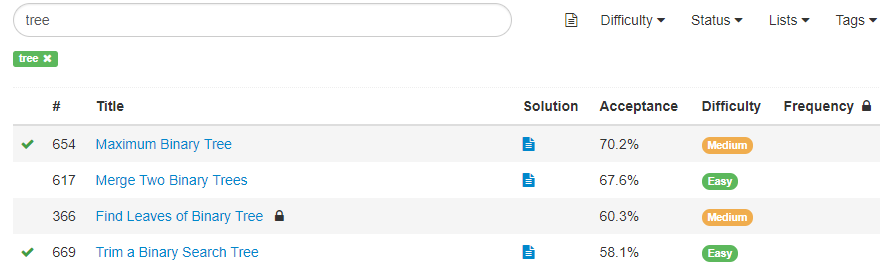
\includegraphics[scale=0.4]{homepageUI}
\caption{The homepage of LeetCode allows users to search for specific types of questions.}
\label{fig:homepage}
\end{figure}

A user simply chooses the question that they wish to attempt, and is promptly brought to the problem's specific screen, as seen in Figure \ref{fig:problemPage}. On this screen there is a general description of the problem and a few examples for more clarification. This page also contains the online editor that the user will operate to attempt the problem. The online editor is intuitive to understand, and as stated has a variety of options for the user to choose from. 
\begin{figure}[h]
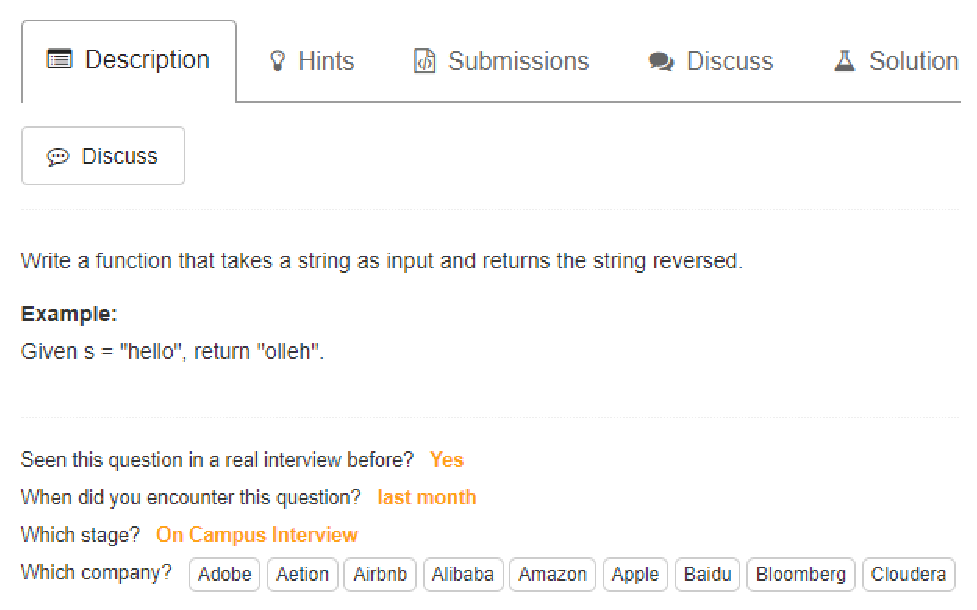
\includegraphics[scale=0.4]{problemPage}
\caption{The question page displays a description of the question and gives a concise example.}
\label{fig:problemPage}
\end{figure}

\begin{figure}[h]
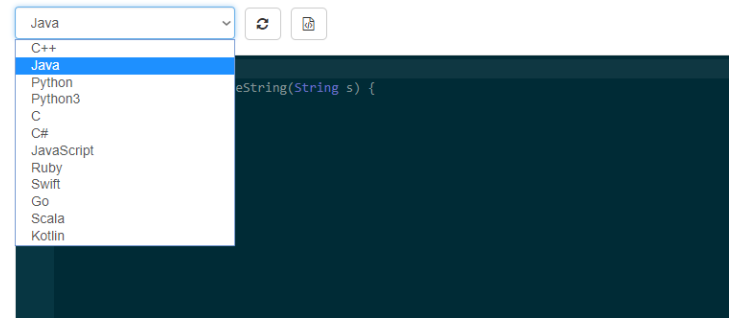
\includegraphics[scale=0.4]{languageUI}
\caption{Online editor with options displayed allowing candidate to use different programming languages.}
\label{fig:langUI}
\end{figure}   
The users attempt to solve the problem they have selected, and they submit their answer and test if it can pass all test cases. They perform this by clicking the submit solution button underneath the editor. LeetCode allows a user to submit their code and be informed almost instantly if they are correct or not. There are two possible outcomes once the user clicks the submit button. Either it is accepted and LeetCode returns an accepted result with suggestions for the next question a user could attempt, shown in Figure \ref{fig:accepted}, or their answer failed a certain test case or even their code failed to compile and run, shown in Figure \ref{fig:fail}. In the case of failure, LeetCode reports where an error is in the code by referencing the line.  
\begin{figure}[h]
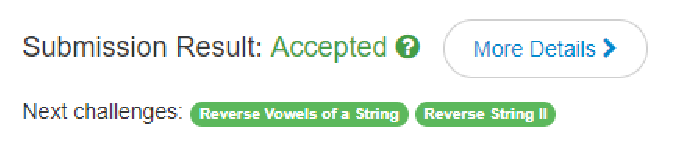
\includegraphics[scale=0.4]{accepted}
\caption{Acceptance message with suggested questions for a user after passing all test cases for a question.}
\label{fig:accepted}
\end{figure}  
\begin{figure}[h]
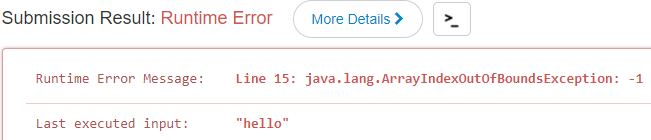
\includegraphics[scale=0.4]{failure}
\caption{Error message after a user submitted a solution for testing.}
\label{fig:fail}
\end{figure}    

\section{Problem Statement}
\label{label:problemstmt}
We formulate the problem statement of this thesis into the following three research questions:
\begin{itemize}
\item \textbf{RQ1: }What algorithms to choose, and what categories are these algorithms associated with. 
\item \textbf{RQ2: }How do these algorithms relate to the fundamental algorithms and how similar are they.
\item \textbf{RQ3: }How easy is it for a person to identify the pattern of the algorithm.
\end{itemize}

\section{The Solution}
To answer RQ1, we first collect useful information. For example, many companies take their questions from online repositories such as LeetCode, and websites that discuss experiences people had at interviews, such as GlassDoor \cite{glassdoor}. We also read through interview preparatory books. These books typically list a range of topics covered in interviews, such as Cracking the Coding Interview covers Binary Search, Dynamic Programming and Graph Traversal \cite{mcdowell2015cracking}. Further many websites publish the top real-world interview questions. This is based on the user interview experience. For example, GeeksforGeeks has a list of the top interview questions that a user should study prior to an interview, for example Linked Lists, Binary Search Trees and Sorting \cite{geeksalgos}. For these reasons, this thesis focuses on the following algorithms:

\begin{table}[H]
\centering
	\begin{tabular}{| c | } \hline
		  {\bf Algorithms} \\ \hline
		Sorting Algorithms\\ \hline
		Searching Algorithms\\ \hline
		Graphs  \\ \hline
		Trees  \\ \hline
		Dynamic Programming \\ \hline
	\end{tabular}
	\caption{Algorithms chosen for this project}
	\label{tab:fiveareas}
\end{table}
In each of these areas we categorise them into seven key patterns (see Table \ref{tab:classicalAlgos}). These are patterns of the listed algorithms that commonly appeared.
\par Among the many websites and interview books, we discovered Leetcode is possibly the best resource for preparing for interviews. Therefore, we select thirty-six questions. These thirty-six questions are representative of the five algorithms in Table \ref{tab:fiveareas}. The questions that we choose are based on online voting and the tags associated with the question. LeetCode's system allows users to vote on questions, indicating that the questions appeared frequently in interviews. We also consider the pass rate and reputation of the question. Relating back to Figure \ref{fig:homepage}, it can be seen that questions can be filtered. Leetcode has over six hundred questions, which is impossible to answer in such a short period of time. 
\par With regards to RQ2, in order to find the most similar algorithm, we first compare the ideas of the standard algorithm and the solution to the question we were solving. It is possible to have multiple algorithms apply to a problem. We implement the easiest solution, this being the first that comes to our minds. This is because one normally has limited time in an interview, and a person builds on an idea they initially discover.
\par To try and obtain a numerical representation of similarity between the standard algorithm and the solution we create, we decide to count how many edit operations we require to transform one piece of code into another. These edits are categorised into two operations, adding and deleting code.
\par As this would be a considerable task to perform by hand, we initially consider an online text comparator called DiffChecker \cite{diff}. DiffChecker returns the number of edit operations required to transform one piece of code into the other. However, we found that DiffChecker fails on a logical level. For example, the same logic structure but with different variable names will be returned as different by DiffChecker. Therefore, these tools can only compare the algorithm on a text level. 
\par Secondly, we consider tools used for plagiarism detection, for example Moss. These tools can be used to detect differences on a logical level. However, using these tools is not easy, as there is a lack of documentation for users and it is laborious to use \cite{mosswebsite}. 
\par Therefore we decide to combine the text comparison and logical comparison approach to form our solution to RQ2. Our approach first judge's similarity by using our own intuition. Secondly, we use control flow graphs (CFG) to manually verify the logic \cite{softwaretesting}. Given the timeframe this is possibly the most suitable approach to make sure this project meets the deadline. Our approach can be seen in the sections that follow. We first display the standard algorithm, then a solution to a question we have judged to be related. Finally, we list the two CFGs for the standard algorithm and the question we have chosen. 
\par Adding or deleting a node or edge was counted as one operation. We choose control flow graphs because they are simple to create and understand. They show the natural flow of the program and this allows for easy evaluation of similarity to a standard pattern. We total the edit operations and if the number is below ten, these two pieces of code were similar. Anything above ten is regarded as being dissimilar.
\par We now present the identified algorithms in Table \ref{tab:classicalAlgos} in the following section. We display the pseudocode for the algorithms and the control flow graphs for each. We display only a few to represent all of the questions due to the page limit. Please see Table \ref{tab:tabSols} for more detail. All the control flow graphs can be found in Appendix B of the Supporting folder of this thesis.
\subsection{Palindrome}
Palindromes are extremely useful for searching. As Palindromes are the same in both directions, one can easily discern if the input is a palindrome. This is helpful for searching as one can search and find any odd characters, or the unique piece of data in some text. This style of algorithm is space efficient. It has a space analysis of $O(n/2)$ as the algorithm works over two elements of the input at a time. The basic approach of a Palindrome algorithm is to work inwards with two pointers starting at either end of the input, moving towards one another and comparing if the elements are the same.\\ 
Algorithm \ref{fig:pal} is a general algorithm for solving the palindrome problem. This approach can be used to solve numerous other problems by altering the inside of the loop.

\IncMargin{1em}
\begin{algorithm}[h]
	\LinesNumbered
	\SetKwInOut{Input}{Input}
	\SetKwInOut{Output}{Output}
	\Input{Given input of characters, S}
	\Output{Boolean}
	$leftIndex  \longleftarrow S[0]$ ; $rightIndex \longleftarrow S.length-1$\\
	\While{leftIndex $<$ rightIndex}{	
		compare leftIndex with rightIndex \\
		\If{leftIndex !=rightIndex}{
			\Return false \\
		}
	 	leftIndex++ \\
		rightIndex++\\
	}
\Return true
\caption{The Palindrome Algorithm}
\label{fig:pal}
\end{algorithm}\DecMargin{1em}
 \par \textbf{ID 1} TwoSum is one example where the palindrome algorithm was used to solve the question. This question is described as: \textit{''Given an array of integers, return indices of the two numbers such that they add up to a specific target. You may assume that each input would have exactly one solution, and you may not use the same element twice.''} Algorithm \ref{fig:twosum} is the solution accepted by LeetCode. In this pseudocode we have highlighted any differences in blue, this is the same for all the following answers.
\IncMargin{1em}
\begin{algorithm}[h]
	\LinesNumbered
	\SetKwInOut{Input}{Input}
	\SetKwInOut{Output}{Output}
	\Input{Array of integers nums, target S}
	\Output{Indices i,j}
	$leftIndex  \longleftarrow S[0]$ ; $rightIndex \longleftarrow S.length-1$\\
	\While{leftIndex $<$ rightIndex}{
	\hlc[cyan!50]{Sort the input array nums\;}\\
	\uIf{\hlc[cyan!50]{nums[leftIndex]+nums[rightIndex] $>$ S}}{
		\hlc[cyan!50]{rightIndex$--$\;}
	}\uElseIf{\hlc[cyan!50]{nums[leftIndex]+nums[rightIndex]$<$S}}{
		\hlc[cyan!50]{leftIndex++\;}
	}\Else{
		\Return\hlc[cyan!50]{ leftIndex, rightIndex\;}
	}
     }\Return 0\;
\caption{LeetCode Q1 TwoSum}
\label{fig:twosum}
\end{algorithm}\DecMargin{1em}\\
Algorithm \ref{fig:twosum} shows the main difference is inside the while loop. The loop guard is still identical, and the core idea found inside the loop is based off the same requirements. The key difference is that the moving of the pointers is not performed at the same time, but rather when certain conditions are met. It can be seen that understanding the need to check the values at the positions, and performing a particular action as a result, is the fundamental idea of both the standard algorithm and the specific solution for Algorithm \ref{fig:twosum}. 
 \par Each node in the graphs represents one or more statements in the source code. The lines of code that they represent are next to each node. With regards to the two graphs, Figure \ref{fig:cfgpal} has six nodes and six edges, a total of twelve. In comparison, Figure \ref{fig:cfgtwosum} has eight nodes and ten edges, a total of eighteen. Therefore, six edit operations are required transform one into the other; two additional nodes and four edges. This result only proved to back up the decision that the answer to TwoSum is analogous to the palindrome algorithm.
 \begin{figure}[h]
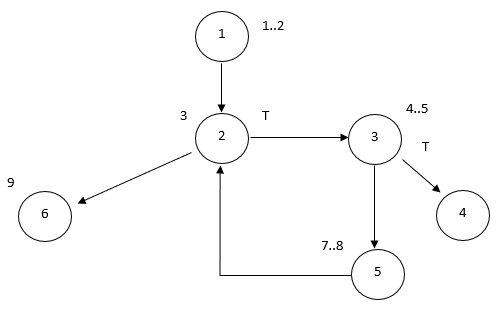
\includegraphics[width=0.6\textwidth]{CFGPalindrome}
\caption{Control Flow Graph for Palindrome}
\label{fig:cfgpal}
\end{figure}
 \begin{figure}[h]
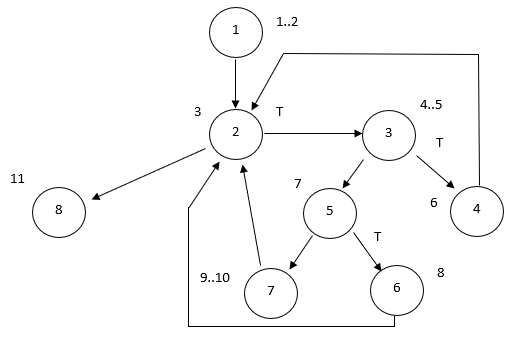
\includegraphics[width=0.6\textwidth]{CFGTwoSum}
\caption{Control Flow Graph for TwoSum}
\label{fig:cfgtwosum}
\end{figure}

\subsection{Merge Sort}
Merge Sort is a very powerful algorithm. It is more efficient than most styles of insertion, with a time analysis of $O(n * log_{n})$, whereas insertion is $O(n^2)$. The idea of merge sort is to divide an array or some input in half and then sort each half before joining it back together. They do not have to be the same size which is useful.  \\
Merge Sort uses the idea of divide and conquer, this means the list to be sorted should be divided up into equal parts first, then these new smaller parts should be sorted individually before recreating the full list. Algorithms \ref{fig:mergesort} and \ref{fig:merge} show this.
\IncMargin{1em}
\begin{algorithm}
	\LinesNumbered
	\SetKwInOut{Input}{Input}
	\SetKwInOut{Output}{Output}
	\Input{List of unsorted data A, int left, int right}
	\Output{Sorted List}
 	\eIf{ left == right}{ \Return A[left]}
  	{$mid \longleftarrow (left+right)/2$\\
  	$recMergeSort(A,left,mid)$\\
  	$recMergeSort(A,mid+1,right)$\\
  	$merge(A,left,mid+1,right)$
  	}
\caption{recMergeSort(). The Merge Sort Algorithm through Recursion}
\label{fig:mergesort}
\end{algorithm}\DecMargin{1em}

\IncMargin{1em}
\begin{algorithm}
	\LinesNumbered
	\SetKwInOut{Input}{Input}
	\SetKwInOut{Output}{Output}
	\Input{List of unsorted data A, int left, int mid, int right}
	\Output{Sorted List A}
 	$n1 \longleftarrow mid - left + 1$ ; $n2 \longleftarrow right - mid$\;
 	$temp1[] \longleftarrow [n1]$  ; $temp2[]\longleftarrow [n2]$\;
 	\tcc*[h]{Copy data into each temparray}
 	\For{$i\leftarrow 1$ \KwTo $n1$}{copy}
	\For{$i\leftarrow 1$ \KwTo $n2$}{copy}
	$i \longleftarrow 0$ ; $j \longleftarrow 0$ ; $k \longleftarrow left$\\
	\While{$i < n1$ \&\& $j < n2$}{
	\If{$temp1[i] <= temp2[j]$ }{
		$A[k] = temp1[i]$; $i++$
	}
	\Else{
		$A[k] = temp2[j]$; $j++$
		}
		$k++$
	}
	\While{$i < n1$}{
		$A[k] = temp1[i]$; $i++$; $k++$
	}
	\While{$j < n2$}{
		$A[k] = temp2[j]$; $j++$; $k++$
	}
	\Return A
\caption{merge(). The merge method for Merge Sort}
\label{fig:merge}
\end{algorithm}\DecMargin{1em}

\par As can be seen, Merge Sort is quite a long algorithm. It contains many intricate parts which must be correct in order for the algorithm to work correctly. \textbf{ID 23} \textit{Merge K Sorted Lists} is an example of Merge Sort being used to solve a problem. 
The question is defined as: \textit{'' Merge k sorted linked lists and return it as one sorted list. Analyze and describe its complexity.''} Algorithms \ref{fig:mergeK} and \ref{fig:mergeK2} are the solution to this question.

\IncMargin{1em}
\begin{algorithm}
	\LinesNumbered
	\SetKwInOut{Input}{Input}
	\SetKwInOut{Output}{Output}
	\Input{ListNode[]A, int left, int right}
	\Output{Sorted List[] A}
 	\eIf{ left == right}{ \Return $A[left]$\;}
  	{$mid \longleftarrow (left+right)/2$\\
  	 \hlc[cyan!50]{$l1 \leftarrow recMergeSort(A,left,mid)$\\}
  	\hlc[cyan!50]{$l2 \leftarrow recMergeSort(A,mid+1,right)$\\}
  	\hlc[cyan!50]{$merge(l1,l2)$}\tcc*[h]{See Algorithm \ref{fig:mergeK2}}\; 
  	}
\caption{recMergeSort() function Merge K Sorted Lists}
\label{fig:mergeK}
\end{algorithm}\DecMargin{1em}

\IncMargin{1em}
\begin{algorithm}
	\LinesNumbered
	\SetKwInOut{Input}{Input}
	\SetKwInOut{Output}{Output}
	\Input{ListNode l1, ListNode l2}
	\Output{Sorted List}
	\If{\hlc[cyan!50]{l1 == null}}{
		\Return \hlc[cyan!50]{$l2$}
	}
	\If{\hlc[cyan!50]{l2 == null}}{
		\Return \hlc[cyan!50]{$l1$}
	}
	\If{\hlc[cyan!50]{$l1.val < l2.val$}}{
		\hlc[cyan!50]{$l1.next = merge(l1.next,l2)$}\\
		\Return \hlc[cyan!50]{$l1$}
	}
	\hlc[cyan!50]{$l2.next = merge(l1,l2.next)$}\\
	\Return \hlc[cyan!50]{$l2$}
\caption{merge() function for \textbf{ID 23}}
\label{fig:mergeK2}
\end{algorithm}\DecMargin{1em}
\par Comparing this solution which is based off of Merge Sort, it can be seen that the main difference is inside the merge method, Algorithm \ref{fig:mergeK2}. On the other hand, Algorithm \ref{fig:mergeK} is very similar to the standard algorithm (Algorithm \ref{fig:mergesort}. Therefore, understanding how to split the data into equal parts is fundamental to both algorithms. It is part of the underlying pattern. The second area for both algorithms is their respective merge methods. Both do differ, this is mainly due to them having different data structures. The key idea that the value of each element of one sub list, should be compared to the other sub list's elements value exists in both Algorithm \ref{fig:merge} and \ref{fig:mergeK2}.
\subsection{Binary Search}
Binary Search is a rapid algorithm for locating data. It has a time complexity of $O(log{n})$ and is used when working with sorted arrays. The algorithm is also used when using binary search trees. In this section the examples are shown with arrays. This algorithm compares the target value to the middle value of the array. If the target is less than this middle value, then the upper half is eliminated as the target cannot lie in this section. The search continues on the remaining half until the search is successful or not. Algorithm \ref{fig:binary} shows the standard Binary Search algorithm.
\IncMargin{1em}
\begin{algorithm}[h]
\LinesNumbered
	
	\SetKwInOut{Input}{Input}
	\SetKwInOut{Output}{Output}
	\Input{Sorted array S, target x}
	\Output{index of target or -1}
	$left \longleftarrow $0 ; $right \longleftarrow S.length-1$\\
	\While{left $<=$ right}{
		$mid \longleftarrow left + (right - left)/2$\\
		\If{S[mid] $==$ x}{
			\Return $mid$
		}
		\If{S[mid]$<$x}{
		$left = mid + 1$
		}
		\Else{
		$right = mid-1$
		}
	}
	\Return -1
\caption{Binary Search}
\label{fig:binary}
\end{algorithm}\DecMargin{1em}

\textbf{ID 69} \textit{Sqrt(x)}, is just one example of Binary Search being employed to solve a question. This question is described as: \textit{''Implement int sqrt(int x). Compute and return the square root of x. x is guaranteed to be a non-negative integer.} Algorithm \ref{fig:sqrt} is the solution to this problem. 
\IncMargin{1em}
\begin{algorithm}
\LinesNumbered
	
	\SetKwInOut{Input}{Input}
	\SetKwInOut{Output}{Output}
	\Input{Int x}
	\Output{Int y}
	\If{\hlc[cyan!50]{x $==$ 0}}{ \Return \hlc[cyan!50]{0}}
	$left \longleftarrow 1$ ; $right \longleftarrow x/2$\\
	\While{true}{
		$mid \longleftarrow left + (right - left)/2$\\
		\If{\hlc[cyan!50]{mid $>$ x/mid}}{
			$right = mid-1$
		}
		\Else{
		\If{\hlc[cyan!50]{$mid+1 > x/(mid+1)$}}{
			\Return \hlc[cyan!50]{$mid$}
			}
			\hlc[cyan!50]{$left = mid+1$}
		}
	}
\caption{Sqrt(x)}
\label{fig:sqrt}
\end{algorithm}\DecMargin{1em}
\par A second example of a question from leetcode.com which is based on Binary Search is \textbf{ID 441} Arranging Coins. The description for this questions is: \textit{''You have a total of n coins that you want to form in a staircase shape, where every k-th row must have exactly k coins. Given n, find the total number of full staircase rows that can be formed. n is a non-negative integer and fits within the range of a 32-bit signed integer.''} Algorithm \ref{fig:arrangingcoins} is the solution to this problem.  
\IncMargin{1em}
\begin{algorithm}
	\LinesNumbered
	\SetKwInOut{Input}{Input}
	\SetKwInOut{Output}{Output}
	\Input{Int n}
	\Output{Number of full steps completed}
	$low\longleftarrow $1 ; $high \longleftarrow $\hlc[cyan!50]{n}\\
	\While{low $<=$ high}{
		$mid \longleftarrow low + (high - low)/2$\\
		\If{\hlc[cyan!50]{mid $*$ (mid+1L) $<=$2L$*$n }}{
			$low = mid+1$\\
		}
		\Else{
			$high = mid -1$\\
	}
}\Return \hlc[cyan!50]{high}\;
\caption{Arranging Coins}
\label{fig:arrangingcoins}
\end{algorithm}\DecMargin{1em}
\par Both of the solutions we present in Algorithm \ref{fig:sqrt} and \ref{fig:arrangingcoins} are extremely close to the original pattern of Binary Search. Both have a calculation to obtain the middle index and both compare the middle index value against the given value using a conditional. Both use a loop structure to cycle through the given data and/or value too. This shows that understanding the need to calculate the middle index and use this for comparisons against the given information will allow a user to solve multiple problems.
%\par As is detailed in Algorithm \ref{fig:arrangingcoins}, this solution is extremely close to the original pattern for binary search. The first change of note is within the assignments at the start. This is where the variable \textit{high} is set to n. This is so the calculation starts at n, as this is the upper limit and max number of steps that could theoretically be produced. The main change required is in the first conditional, which when returns true means that the lower side must be moved up, so \textit{low} is reset to be mid + 1.
\par The total number of nodes in the original pattern is eight and it contains nine edges. In the specific version for Arranging Coins there are a total of six nodes and seven edges. The total is therefore four edit operations required to transform between the two pieces of source code.
 \begin{figure}[H]
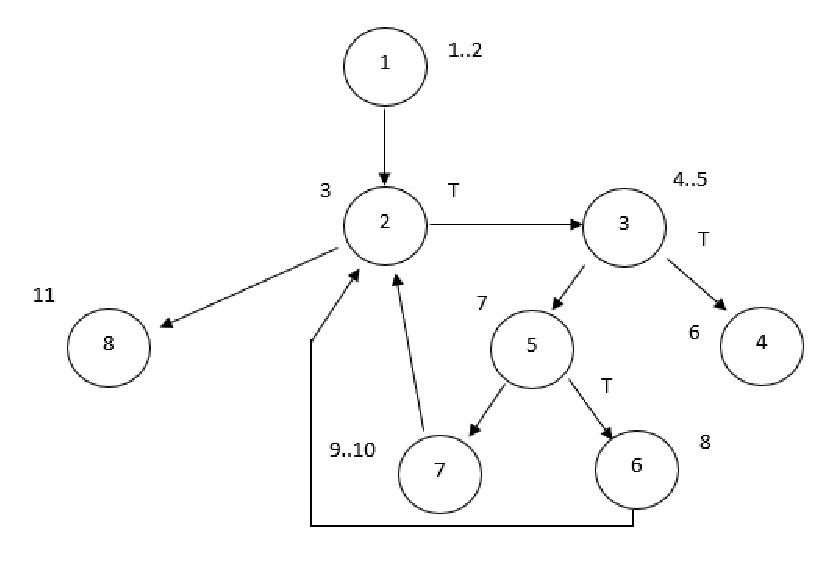
\includegraphics[width=0.6\textwidth]{CFGBinarySearch}
\caption{Control Flow Graph for Binary Search}
\label{fig:cfgbinarysearch}
\end{figure}
 \begin{figure}[H]
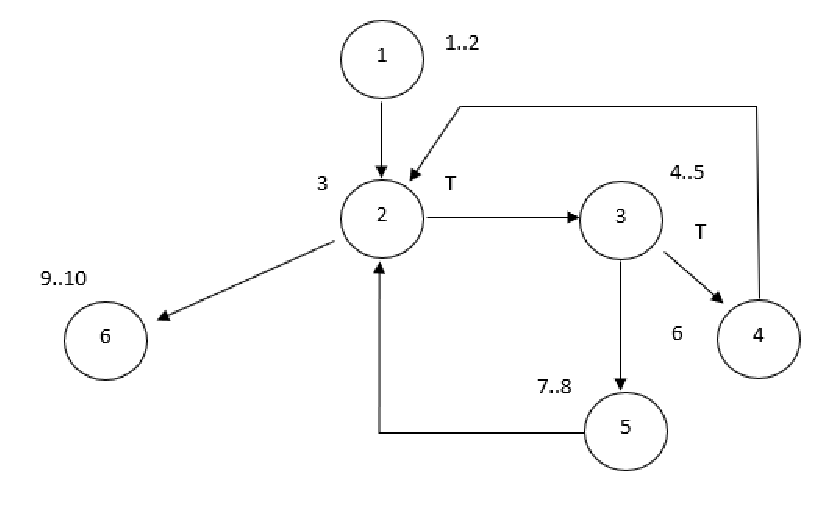
\includegraphics[width=0.6\textwidth]{CFGArrangingCoins}
\caption{Control Flow Graph for Arranging Coins}
\label{fig:cfgbinarysearch}
\end{figure}

	
	\subsection{Graphs}
	Graphs are common in our lives. Graphs studied by Computer Scientists are usually based on the tree structure, and the relationships among data elements. A tree is just one of the special types of graphs that can be studied, where the parent-child relationship is used to organise data. In this section we focuse on the Tree Abstract Data Type, Breadth-First Traversal and Graphs in general. \\
	\subsubsection{Trees}
	Trees are one of the most powerful styles of data structures for processing data. They allow rapid searching and fast insertion/deletion of a node. Trees are made up of nodes, which are objects which hold some data and have a key. This key allows one to determine where this node should be in the tree. These nodes contain references to children instead of just the next Link. Each node has exactly one parent, but can have many children. A Binary Search Tree is a special type of tree. It has strictly between zero and two children, and keeps their keys in sorted order. It has $O(n)$ space, search, insertion and deletion operations. 
	\par With trees the main function is traversal. There are three basic styles of traversal: inorder, preorder and postorder. Inorder visits every node in the left subtree, then the root and finally the right subtree. Preorder visits the root first, followed by the left subtree and then the right subtree. Finally, postorder is where the left subtree is followed by the right subtree and then the root. 
\par Algorithm \ref{fig:nodesearch} is an example of how one might search for a particular node in a Tree. Algorithm \ref{fig:postorder} is the basic postorder traversal of a tree. The key area to note is the order of calling the different children of a node. Altering this will result in preorder and inorder traversal.
\IncMargin{1em}
\begin{algorithm}
	\LinesNumbered
	\SetKwInOut{Input}{Input}
	\SetKwInOut{Output}{Output}
	\Input{Given a key to search for}
	\Output{The desired Node, or null}
	$Node$ $current$ $\longleftarrow root$\;
	\While{$current.data != key$}{
		\If{$current == null$}{\Return $null$}
		\eIf{$current.data > key$}{
			$move$ $left$ $on$ $the$ $tree$\\
		}{
		$move$ $right$ $on$ $the$ $tree$\\
		}
	}
\Return $current$\;
\caption{Finding a specific Node in a tree based on the key}
\label{fig:nodesearch}
\end{algorithm}\DecMargin{1em}
\\
\IncMargin{1em}
\begin{algorithm}
\SetAlgoNoLine
\LinesNumbered
	\SetKwFunction{postOrder}{postOrder}
	\Indm\postOrder{$Node$ $localRoot$}\\
		\If{localRoot $!=$ null\\}{
		$\postOrder(localRoot$ $leftChild)$\\
		$\postOrder(localRoot$ $rightChild)$\\
		$Print(localRoot$ $data)$}	
\caption{Basic Tree Traversal using PostOrder Traversal}
\label{fig:postorder}
\end{algorithm}\DecMargin{1em}

\par \textbf{ID 104}, \textit{Maximum Depth of Binary Tree}, is an example of a question where the basic tree traversal styles were used to solve the question. The problem description is given as: \textit{''Given a binary tree, find its maximum depth. The maximum depth is the number of nodes along the longest path from the root node down to the farthest leaf node.''} Postorder traversal was used. Algorithm \ref{fig:maxdepth} details the solution.
\IncMargin{1em}
\begin{algorithm}
\SetAlgoNoLine
\LinesNumbered
	\SetKwFunction{maxDepth}{maxDepth}
	\Indm\maxDepth{$TreeNode$ $localRoot$}\\
		\If{\hlc[cyan!50]{localRoot $==$ null}}{\Return \hlc[cyan!50]{0\;}}
		\Else{
		\hlc[cyan!50]{$ldepth$}=$\maxDepth(localRoot leftChild)$\\
		\hlc[cyan!50]{$rdepth$}=$\maxDepth(localRoot rightChild)$\\
		\If{\hlc[cyan!50]{ldepth $>$ rdepth}}{
		\Return  \hlc[cyan!50]{$ldepth+1$\\}
		}\Else{ \Return \hlc[cyan!50]{$ rdepth+1$\\}}
		}
\caption{Leetcode Q104 Max. Depth of Binary Tree}
\label{fig:maxdepth}
\end{algorithm}\DecMargin{1em}
\\
\par The similarities between Algorithms \ref{fig:maxdepth} and \ref{fig:postorder} are that in each case we recursively traverse down the left branch of the tree, followed by the right branch and finally we consider the root node. The key idea to understand from the original algorithm is that by traversing down one branch at a time, the user can obtain the longest path in the tree. By initially going down the left and only the left, the user can obtain the value for this branch. When this left branch of the tree has been completely searched and the path value stored, then and only then will the right branch be traversed in the same manner. Therefore, having the knowledge that traversing a tree in a specific way can give a user information is vital and what the user should aim to understand with tree traversal patterns.  
\par This similarity is only reinforced when the CFGs are considered. Figures \ref{fig:cfgpostorder} has four nodes and 6 edges, Figure \ref{fig:cfgmaxdepth} has five nodes and five edges. Therefore, they have an identical total of ten. This shows the two algorithms are closely related, as detailed in the previous paragraph.
 \begin{figure}[h]
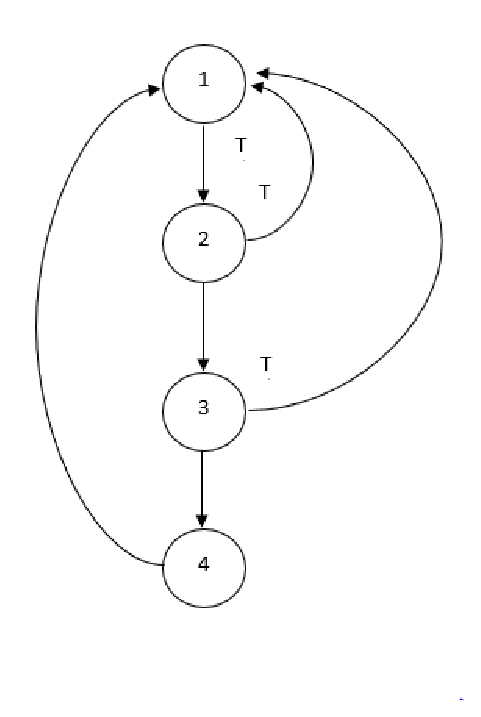
\includegraphics[scale=0.4]{CFGPostOrderAlg11}
\caption{Control Flow Graph for postorder}
\label{fig:cfgpostorder}
\end{figure}

\begin{figure}[h]
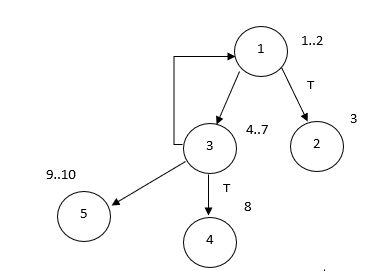
\includegraphics[scale=0.4]{CFGMaxDepthAlgo12}
\caption{Control Flow Graph for Max Depth}
\label{fig:cfgmaxdepth}
\end{figure}
\subsubsection{Breadth-First Search}
This is a special traversal pattern. The ordering visits the root node, then move onto the children of the root node, printing each child in turn. It then will repeat this for each child of these nodes. Figure \ref{fig:breadth} shows the nodes in numerical order of visitation.
\begin{figure}[h]
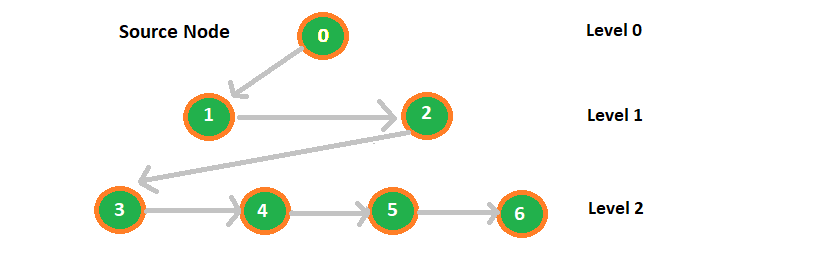
\includegraphics[scale=0.5]{bfs}
\caption{Breadth-First Search. The grey arrows indicate the traversal path.}
\label{fig:breadth}
\end{figure}
 
\subsubsection{Depth-First Search}
This pattern involves starting at the root, then going to the left most child, repeating this movement until the traversal reaches a leaf node, then it will move back up one node and try to visit the next child node. It repeats this until the traversal finds no unvisited node.


\subsection{Dynamic Programming}
Dynamic Programming is outlined as `smart recursion'. This is because it takes the idea of recursion and improves on the inefficiencies of recursion. These inefficiencies mainly being that recursive algorithms are generally space inefficient. Each recursive call adds a new layer to the stack. Therefore, dynamic programming is such a strong style of programming as it uses the simplicity of recursion but does not have the problem of causing a stack overflow. Dynamic programming is described as taking a recursive algorithm and finding the overlapping subproblems. A user then caches these results for future recursive calls.
This style is known as \textit{Top-Down}. There is a different approach, known as \textit{Bottom-Up}. We give a quick demonstration of the two by using the classic recursive algorithm to solve Fibonacci numbers.
\IncMargin{1em}
	\begin{algorithm}
	\LinesNumbered
		%\Fn(\tcc*[h]{recursive fibonacci}){\FRecurs{Integer n}}{
		\SetKwInOut{Input}{Input}
		\SetKwInOut{Output}{Output}
		
		\Input{Integer n}
		\Output{Fibonacci Numbers}
		\If{n$<$3} {\Return 1\\}
		\Return $fib(n-2) + fib(n-1)$
			
	\caption{Fibonacci Numbers through normal recursion}
	\end{algorithm}
\DecMargin{1em}
	
	\subsubsection{Top-Down}
	This method of dynamic programming follows the normal structure of a simple recursive solution. Start from n and compute smaller results as they are needed to solve the original problem. Results are stored in some form of data structure, this is known as memoization. These stored results are accessed efficiently in comparison to having to recompute the same values for n repeatedly. See Algorithms \ref{fig:topdown1} and \ref{fig:topdown}.
\IncMargin{1em}
	\begin{algorithm}
	\LinesNumbered
		\SetKwInOut{Input}{Input}
		\SetKwInOut{Output}{Output}
		\Input{Integer n}
		\Output{Fibonacci Numbers}
		$computed \leftarrow $HashMap\;
		\If{n$<$3} {\Return 1\\}
		\Return $fib(n-2) + fib(n-1)$\\
		$computed put (1,1)$\\
		$computed put (2,1)$\\
		\Return $fib2(n, computed)$\\
		\caption{fib; Fibonacci Numbers through Top-Down and Memoization}
		\label{fig:topdown1}
	\end{algorithm}\DecMargin{1em}
\IncMargin{1em}
	\begin{algorithm}
	\LinesNumbered
		\SetKwInOut{Input}{Input}
		\SetKwInOut{Output}{Output}
		\Input{Integer n, HashMap computed}
		\Output{Fibonacci Number}
		\If{computed containsKey(n)} {\Return $computed get(n)$\\}
		$computed.put(n-1,fib2(n-1,computed))$\\
		$computed.put(n-2,fib2(n-2,computed))$\\
		$newVal \leftarrow computed.get(n-1) + computed.get(n-2)$\\
		\Return $newVal$\\
	\caption{fib2;Fibonacci Numbers through Top-Down and Memoization}	
	\label{fig:topdown}
	\end{algorithm}\DecMargin{1em}	
	
	\subsubsection{Bottom-Up}
	The issue with the Top Down version is that even though the results are being saved to reuse later, they must be calculated from n to the base cases through recursion the first time. This is performed only once, when no values have been computed.
	Bottom-Up solves this by starting at the base cases and computing until it reaches the value of n. See Algorithm \ref{fig:bottomup}.
\IncMargin{1em}
	\begin{algorithm}
	\LinesNumbered
		\SetKwInOut{Input}{Input}
		\SetKwInOut{Output}{Output}
		\Input{Integer n}
		\Output{Fibonacci Numbers}
		\SetKwArray{Kw}{results}
		$results[] \leftarrow int[n+1]$ ; $results[1] = 1$ \\ $results[2] = 2$ \\
		\For{$i \leftarrow 3$ \KwTo $n$}{ 
		$results[i] = results[i-1]+results[i-2]$\\}
		\Return $results[n]$\\		
		\caption{fibDP; Fibonacci Numbers through Bottom-Up}
		\label{fig:bottomup}
	\end{algorithm}\DecMargin{1em}
	\\
\par It must be noted that Dynamic Programming is one of the toughest sections of programming to learn. This only makes it more challenging for candidates to answer questions in such a limited window. The reason it is tough is because a candidate must think of the problem in multiple ways, and make the decision to tackle it in a certain manner. If they choose the wrong option, then they will end up with an inefficient solution. Choose correctly and they will have shown a very strong understanding of this area.\\

 The important aspect of this pattern is storing the calculated information in a data structure. It therefore allows for rapid lookup and less calculations to be on the stack at any given time. 
\section{Evaluation}
In the previous section of this thesis, only specific examples of the solutions were shown. Here we give a detailed summary of all solved questions in Table \ref{tab:tabSols}. The solutions to these questions passed all test cases and were accepted by LeetCode's online judging system. We also create a table for the algorithms previously listed in the solution section, and a table for the data structures used in their solutions, Table \ref{tab:classicalAlgos}.
\begin{table}
\parbox{.45\linewidth}{
\centering
\begin{tabular}{|c|c|} \hline
		    & {\bf Algorithms} \\ \hline
		1 & Palindrome\\ \hline
		2 & Merge Sort\\ \hline
		3 & Binary Search\\ \hline
		4 & Tree Traversal \\ \hline
		5 & Breadth-First Search\\ \hline
		6 & Depth-First Search\\ \hline
		7 & Dynamic Programming\\ \hline
		- & None required\\ \hline
\end{tabular}
\caption{The standard algorithms and data structures}
\label{tab:classicalAlgos}
}
\hfill
\parbox{.45\linewidth}{
\centering
\begin{tabular}{|c|c|} \hline
	&{\bf Data Structures} \\ \hline
	1 & List\\ \hline
	2 & Trees\\ \hline
	3 & Stacks\\ \hline
	4 & Queues \\ \hline
	5 & Arrays\\ \hline
	6 & Maps\\ \hline	
	7&Strings\\ \hline
	-&None required\\ \hline
\end{tabular}
}

\end{table}

\begin{table*}
\begin{tabular}{|c| c| c| c| c| c|} \hline
 {\bf Question ID} & {\bf PassRate} & {\bf Difficulty} & {\bf Time(in minutes)} & {\bf Evaluation} & {\bf Algorithm Pattern} \\
	 \hline
 	1 & 36.0\% & Easy & 9 & Easy & [1,[5]]\\ 
 	\hline
	 2 & 28.1\% & Medium & 20 &Medium& [-.[1]]\\
 	\hline
	 20 & 33.7\% & Easy & 12&Easy& [1,[3]] \\
 	\hline
 	21 & 39.3\% & Easy & 25&Easy& [-,[1]] \\
 	\hline
 	23 & 27.7\% & Hard & 27&Medium&[2,[1,5]] \\
  	\hline
 	35 &39.8\%  & Easy & 10 &Easy&[-,[5]]\\
  	\hline
 	53 &39.9\%  & Easy & 20 &Medium& [-,[5]]\\
  	\hline
 	58 & 32.0\% & Easy & 15 &Easy&[-,[5,7]]\\
  	\hline
 	69 & 28.2\% & Easy & 19 &Easy&[3,[-]]\\
  	\hline
 	70 & 40.5\% & Easy & 18 &Easy&[7,[5]]\\
 	\hline
 	72 & 32.1\% & Hard & 29 &Hard&[7,[5]]\\
  	\hline
 	88 & 32.1\% & Easy & 12 &Medium&[-,[5]]\\
  	\hline
 	94 & 47.8\% & Medium & 27 & Medium&[4,[1,2,3]]\\
  	\hline
 	102 & 40.9\% & Medium & 30  &Medium & [5,[1]]\\
  	\hline
	104 & 53.5\% &Easy  &28  &Medium& [4,[2]]\\
  	\hline
 	111 &  33.3\%& Easy&17  &Easy& [5,[2,4]]\\
  	\hline
 	114 & 35.7\% &Medium  & 33  &Medium&[4,[2]]\\
  	\hline
 	136 &54.9\%  &Easy  &10  &Easy& [-,[5]]\\
  	\hline
 	147 & 33.4\% &Medium  &26  &Medium& [-,[1]]\\
	\hline
 	152 &  26.2\%& Medium & 31 &Hard&[7,[5]]\\
  	\hline
  	167 & 47.1\% &Easy  &16  &Easy&[1,[5]]\\
  	\hline
  	169 & 47.3\% &Easy  &20  &Easy&[-,[5]]\\
  	\hline
  	205 & 34.2\% &Easy  &18  &Easy& [-,[6]]\\
  	\hline
  	230 & 44.1\% &Medium  &19  &Medium&[4,[2,3]]\\
  	\hline
 	290 & 33.2\% &Easy  &28  &Medium&[-[5,6]]\\
  	\hline
 	326 & 40.4\% &Easy  &25  &Easy&[-[-]]\\
   	\hline
  	336 & 26.5\% &Hard &18  &Medium&[1,[1,7]]\\
  	\hline
 	344 & 59.5\% &Easy  &8  &Easy&[1,[5,7]]\\
  	\hline
 	387 & 47.1\% &Easy  & 19 &Medium&[-,[5]]\\
  	\hline
 	389 & 50.9\% &Easy  & 10 &Easy& [-,[5]]\\
  	\hline
 	404 & 47.3\% &Easy  &16  &Medium&[4,[2]]\\
	\hline
 	441 & 36.3\% &Easy  &6&Easy &[3,[-]]\\ 	
  	\hline
 	654 & 70.1\% &Medium  &46  &Hard&[2,[2,5]]\\
  	\hline
	669 &  58.1\%& Easy &18  &Easy&[4,[2]]\\
  	\hline
	687 &  33.5\%& Easy &21  &Medium&[-,[2]]\\
  	\hline
 	690 &  52.9\%& Easy &   45&Medium&[5,[3,6]]\\[1ex]
 	\hline
\end{tabular}
\caption{Total of 36 solutions we analysed for this project}
\label{tab:tabSols}
\end{table*}
\par In Table \ref{tab:tabSols}, \textit{Question ID} indicates a specific ID of LeetCode question we solved. \textit{PassRate} is the percentage of solutions accepted by LeetCode. These were taken at the time of writing. \textit{Difficulty} is the level that was awarded to each question by LeetCode. \textit{Time} is the total time in minutes it took to complete each question. \textit{Evaluation} is our opinion on the difficulty of each question. \textit{Algorithm Pattern} implies that the algorithms and data structures pattern we identify and are similar to the standard algorithms in Table \ref{tab:classicalAlgos}. Each pattern is enclosed in a list. The first component in this list is a number that refers to a similar standard algorithm. The second component is a list that refers to the relevant data structures (in Table \ref{tab:classicalAlgos}) used . For example, $[4,[2]]$ means it uses \textit{Tree Traversal} (from algorithm 4 in Table \ref{tab:classicalAlgos}) and \textit{tree} data structure from Table \ref{tab:classicalAlgos}. For the source code of each solution listed in Table \ref{tab:tabSols}, please view our online repository:
\begin{center}
\url{https://github.com/Demostroyer/interview-project/}
\end{center}
\par As can be seen in Table \ref{tab:tabSols}, some of the questions that are marked as having difficulty \textit{easy}, took longer than some that are marked as \textit{medium}. This is because it takes longer for the pattern that is useful to solve the problem to be discovered.
\par To answer RQ3 we describe the different types of users that potentially will prepare interview questions. It is not easy to judge how fast a user can detect the underlying pattern of a problem. This is because each user will have a different background. We have categorised the different users into four distinct types. 
\begin{enumerate}
\item{People which have a background in coding competitions. They are highly experienced and unlikely to find the questions hard.}
\item{Users with some computer science background, who understand the internal workings of data structures and other concepts. These people would find most problems approachable.}
\item{People who understand basic concepts. They will struggle with the advanced topics.}
\item{People who are interested in learning to code who have no experience. They will have to put a lot of study in to grasp basic concepts.}
\end{enumerate}
This leads to the creation of Table \ref{tab:difficulty}. Here each type of user is paired with the expected difficulty they would face answering the questions on LeetCode. 

\begin{table}[H]
\centering
	\begin{tabular}{| c | c |} \hline
		  {\bf Background Type} &{\bf Expected Difficulty} \\ \hline
		1 & Easy \\ \hline
		2 & Medium \\ \hline
		3 & Medium  \\ \hline
		4 & Hard  \\ \hline
	\end{tabular}
	\caption{The expected difficulty each type of categorised user would have with the questions}
	\label{tab:difficulty}
\end{table}

\subsection{Question Evaluation}
Whilst working on the numerous questions, some issues did arise that related to the questions themselves. These problems stem from the questions being worded abnormally, or the example given for the solution not being explicitly clear in the way the question operated. These were just some of the issues that occurred whilst attempting to solve the problems. An example of such an issue is \textbf{ID} 654, Maximum Binary Tree. This question's problem was easy to understand:
\\ \textit {''Given an integer array with no duplicates. A maximum tree building on this array is defined as follow:
\begin{enumerate}
\item The root is the maximum number in the array.
\item The left subtree is the maximum tree constructed from left part subarray divided by the maximum number.
\item The right subtree is the maximum tree constructed from right part subarray divided by the maximum number.
\end{enumerate}
Construct the maximum tree by the given array and output the root node of this tree''.}\\
The issue that we personally came across was trying to understand the way the left and right subtree should be structured. The description for them was not clear, as we were unsure what was meant by $''$left part subarray divided by the maximum number$''$. The provided example is as follows.
\begin{figure}[h]
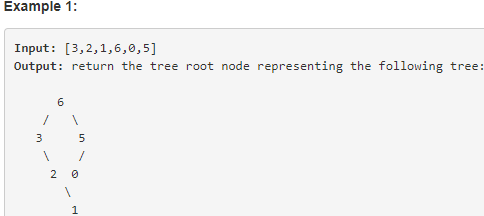
\includegraphics[scale=0.5]{example654}
\caption{Unclear example for ID 654}
\end{figure} \\
This did not make it any clearer. It was simple to understand that the biggest number in the subarray should be the next number in the tree and to work in a descending manner. What is hard to understand is the two being the right child of the three, and yet zero was to the left of five, where it was to be expected. This confusion caused a delay in the solution to this question being completed.

%\par The control flow graphs for each solution is provided in the appendix of this thesis. Each of these graphs starts at the method signature of each method which solves the question. Therefore, the line number associated with the first node starts at line one, regardless of the line in the source code. The inline comments are also discounted when generating the graphs.

\section{Limitations}
 There are two limitations in this thesis. 
 
 Firstly, the topics that are covered are only a selection of algorithms, there are many more to be studied. For example, the questions focusing on \textit{Insertion Sort} were never formally addressed in this thesis. This can be improved by solving more algorithms from more topics.
 
 Secondly, our approach has its limitations. It was manual, meaning it was dependent on the ability of us as programmers. This meant that our ability to solve some questions was stronger on certain topics than others. For example, the questions relating to the advanced topic Dynamic Programming took longer to learn and therefore, took longer to complete. This is due to this section being an advanced area. As this approach was manual, there was a lot of human effort required. This results in questions taking longer than expected to be completed, and questions being solved in ways that might not be the most optimal. This can be solved by developing some form of automatic validator.

\section{Related Work}
As was mentioned earlier in this thesis, there are some pieces of literature that focus on analogous topics. These include books that aim to give solutions to common programming questions \cite{mcdowell2015cracking} and the fundamentals of java \cite{markham2014java}\cite{aziz2012elements}. There are also some websites that have some mock interview questions and stage the mock interview to be like the normal interview process by having limited time and selected questions \cite{pramp}.
\par With regards to our approach to finding similarity between the algorithm and solution, there are a number of related works that we have previously mentioned. These being DiffChecker for text comparison and Moss for plagiarism checking. 
\par DiffChecker works by comparing each letter inside the text. It returns any discrepancies found whilst scanning through the text. The issue is that this will return pieces of the text that are logically the same but textually different. In comparison to our approach of using control flow graphs, this is not accurate enough. 
\par Moss is a powerful tool for detecting plagiarism. Moss is described as an automatic system for determining the similarity of programs \cite{mosswebsite}. The tool itself is heavily focused on finding plagiarised pieces of code from given sources. Moss uses a technique known as robust winnowing. Winnowing is a technique normally found in machine learning and document fingerprinting \cite{Schleimer:2003:WLA:872757.872770}. This approach is strong, but slow in practice. In terms of the time frame given for this project, we decided it is better to perform the logical check manually. This is achieved by using control flow graphs.

\section{Conclusion and Future Works}
In this thesis we have created a guide for beginners in programming, fresh graduates and readers who wish to refresh their knowledge. This enables them to learn and understand some of the fundamental algorithms of programming quickly. Through learning these patterns the reader should be able to identify solutions to a wide array of coding problems. 
\par The approach taken in this thesis was to solve each question manually. This means the solutions were all attempted and completed by a human. Therefore, this process was similar to the interview environment. This is due to both the interview and approach taken for this thesis, having the human element of thinking of multiple ways to tackle the issues. This allowed the approach to be as valid and authentic to the real scenario of the interview as possible.
In this thesis there was no automatic approach to solving the questions developed. This would have been helpful for validating the solutions produced by the manual methodology. This automatic process was unable to be produced because of the time constraints. 

This thesis serves as a pilot study for future improvement. In the future, we plan to use machine learning techniques to predicate a possible algorithmic pattern and data structures to be used to solve a given interview question. This could allow interviewers and candidates to further improve the quality of interview preparation.


\nocite{goodrich2014data,carrano2003data,MossBowyer,VKuncak,Karp:1987,Ragkhitwetsagul2017,Chilowicz,gitHUb}

\bibliography{mybib}
\bibliographystyle{ieeetr}
\end{document}